\documentclass[10pt]{article}
\usepackage[a4paper, tmargin=0.75in, lmargin=0.80in, rmargin=0.80in, bmargin=1in]{geometry}
\usepackage{hyperref}
\usepackage{booktabs}
\usepackage{siunitx}
\usepackage{graphicx}
\usepackage{natbib}
\usepackage{tikz}
\usepackage{float}
\usepackage{xcolor}
\usepackage{amsmath}
\usepackage{array}
\usepackage{tabularx}
\usepackage{listings}
\usepackage{subcaption}
\pagestyle{empty}

%%%%%%%%%%%%%%%%%%%%%%%%%%%%%%%%%%%%%%%%%%%%%%%%%%
% IMAGE TOGGLE + SNAPSHOT PATH
%%%%%%%%%%%%%%%%%%%%%%%%%%%%%%%%%%%%%%%%%%%%%%%%%%
\newif\ifshowimages
\showimagestrue
\ifdefined\NOIMAGES
  \showimagesfalse
\fi
\graphicspath{{report-draft-1/snapshots-26/}}

%%%%%%%%%%%%%%%%%%%%%%%%%%%%%%%%%%%%%%%%%%%%%%%%%%
% UPPAAL QUERY LISTING STYLE (verbatim-like)
%%%%%%%%%%%%%%%%%%%%%%%%%%%%%%%%%%%%%%%%%%%%%%%%%%
\lstdefinestyle{uppaal}{
  basicstyle=\ttfamily\small,
  columns=fullflexible,
  breaklines=true,
  frame=single,
  showstringspaces=false,
  aboveskip=0.5\baselineskip,
  belowskip=0.5\baselineskip,
  literate={_}{{\_}}1
}

%%%%%%%%%%%%%%%%%%%%%%%%%%%%%%%%%%%%%%%%%%%%%%%%%%
% INFORMATION MACROS
%%%%%%%%%%%%%%%%%%%%%%%%%%%%%%%%%%%%%%%%%%%%%%%%%%
\newcommand{\studentname}{Shu-Lin Shih and Jaideep Khare}
\newcommand{\studentnumber}{35199856 and 35193853}
\newcommand{\coursename}{ECE 622: Modeling \& Verification of Embedded Systems}
\newcommand{\semester}{Spring 2026}

%% Viking name: Vik with subscript index (e.g. Vik_1)
\newcommand{\Vik}[1]{\ensuremath{\mathrm{Vik}_{#1}}}

%% Space after an italic prompt before the answer text
\newcommand{\afterprompt}{\par\medskip}

%% Optional width as fraction of \textwidth (default 0.82)
\newcommand{\labfigure}[4][0.82]{%
\begin{figure}[H]
\centering
\ifshowimages
  \includegraphics[width=#1\textwidth]{#2}
\else
  \fbox{\begin{minipage}[c][45mm][c]{0.90\textwidth}
  \centering
  Image omitted in no-image build\\
  \texttt{\detokenize{#2}}
  \end{minipage}}
\fi
\caption{#3}
\label{#4}
\end{figure}
}

\begin{document}

\begin{center}
{\huge{\coursename}} \\
\vspace{2mm}
{\Large{\semester: Lab 2: Verification of Timed Automata using UPPAAL}}\\
\vspace{1mm}
{\Large{Prof. Daniel Holcomb}}
\end{center}

\vspace{5mm}
\hrule
\vspace{1mm}
\hrule

\vspace{3mm}
\begin{tabular}{ll}
Submitted by:  & {\studentname} \\
Student ID:     & {\studentnumber} \\
Lab No.:        & 2 \\
Submission Date:& March 2026 \\
\end{tabular}

\vspace{3mm}
\hrule
\vspace{1mm}
\hrule

\section*{Overview}
This report presents model construction, simulation, and symbolic verification for Lab~2 using UPPAAL. Part~A analyzes timed automata for the Viking bridge-crossing problem under increasingly complex scenarios. Part~B develops and verifies a timed traffic-light and pedestrian-control system, including safety analysis and a robustness extension required for ECE~622.

The workflow used in all sections was: (1) encode model changes in UPPAAL templates/system declarations, (2) state explicit verification queries, (3) run verifier checks, and (4) inspect symbolic or concrete traces to extract schedules and explain results.

\section{Part A: Bridge-Crossing Timed Automata}

\subsection*{A.1: Four Vikings within 60 minutes}
\textit{Determine whether all four Vikings with crossing times \SI{5}{min}, \SI{10}{min}, \SI{20}{min}, and \SI{25}{min} can reach the safe side within \SI{60}{min}, and provide a valid schedule.}
\afterprompt
Model checking query:
\begin{lstlisting}[style=uppaal]
E<> Vik_1.safe && Vik_2.safe && Vik_3.safe && Vik_4.safe && time <= 60
\end{lstlisting}
The query is satisfiable, so a feasible execution exists.

Witness schedule from trace:
\begin{table}[H]
\centering
\begin{tabular}{c >{\raggedright\arraybackslash}p{0.38\textwidth} c c}
\toprule
\# & Trip (Vikings by index; times in minutes) & Start time (\si{min}) & Trip origin \\
\midrule
1 & $\Vik{1}+\Vik{2}$ cross to safe side (5+10) & 0 & Unsafe side \\
2 & $\Vik{1}$ returns with torch (5) & 10 & Safe side \\
3 & $\Vik{3}+\Vik{4}$ cross to safe side (20+25) & 15 & Unsafe side \\
4 & $\Vik{2}$ returns with torch (10) & 40 & Safe side \\
5 & $\Vik{1}+\Vik{2}$ cross to safe side (5+10) & 50 & Unsafe side \\
\bottomrule
\end{tabular}
\caption{A.1 crossing schedule (total completion time: \SI{60}{min}).}
\label{tab:a1_schedule}
\end{table}

The schedule completes all crossings at minute~60, satisfying the time bound exactly.

\begin{figure}[H]
\centering
\ifshowimages
  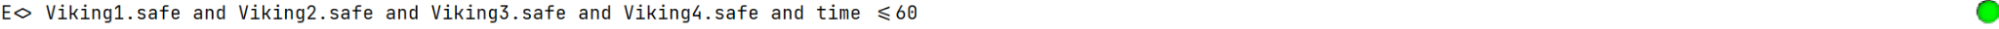
\includegraphics[width=1.0\textwidth,height=0.825\textheight,keepaspectratio]{PartA-1-proof.png}
\else
  \fbox{\parbox[c][55mm][c]{0.98\textwidth}{\centering Image omitted (A.1 proof)}}
\fi
\caption{A.1: UPPAAL verifier for bounded reachability within \SI{60}{min} (displayed at 1.5$\times$ prior proof scale, width $\le$ text width).}
\label{fig:parta_a1_proof}
\end{figure}

\begin{figure}[H]
\centering
\begin{subfigure}[t]{0.48\textwidth}
\centering
\ifshowimages
  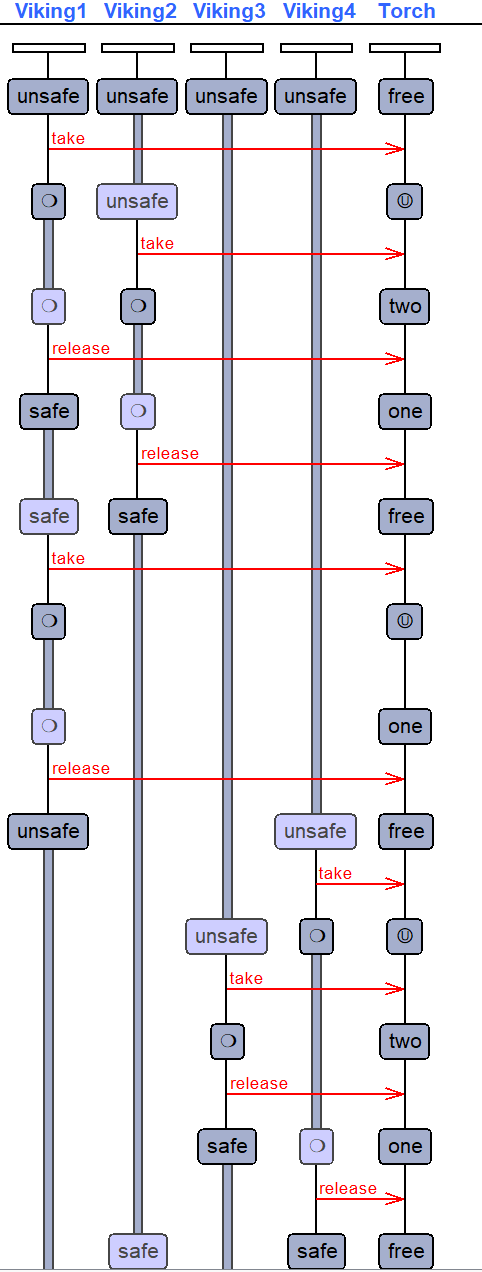
\includegraphics[width=\linewidth,height=0.65\textheight,keepaspectratio]{PartA-a1-img1.png}
\else
  \fbox{\parbox[c][45mm][c]{\linewidth}{\centering omitted}}
\fi
\caption{First segment.}
\label{fig:parta_a1_first}
\end{subfigure}\hfill
\begin{subfigure}[t]{0.48\textwidth}
\centering
\ifshowimages
  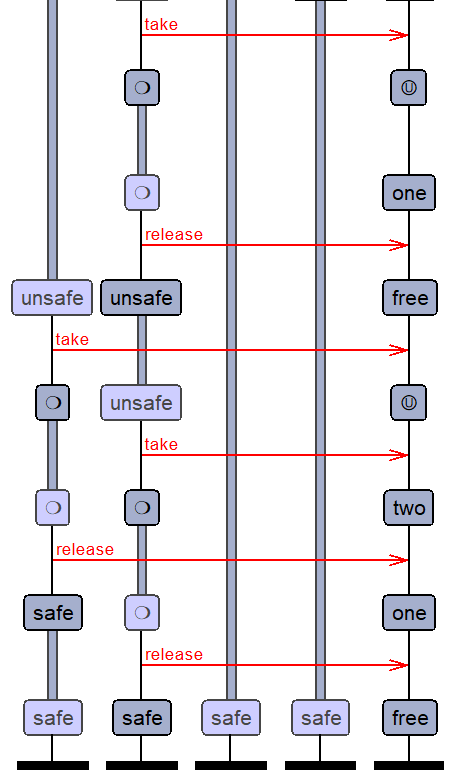
\includegraphics[width=\linewidth,height=0.65\textheight,keepaspectratio]{PartA-a1-img2.png}
\else
  \fbox{\parbox[c][45mm][c]{\linewidth}{\centering omitted}}
\fi
\caption{Second segment.}
\label{fig:parta_a1_second}
\end{subfigure}
\caption{A.1: UPPAAL verifier/trace views for bounded reachability within \SI{60}{min} (two panels).}
\label{fig:parta_a1_strip}
\end{figure}

\subsection*{A.2: Add a fifth Viking (10 minutes)}
\textit{A fifth Viking is added with a \SI{10}{min} bridge delay (in addition to the existing \SI{10}{min} Viking). What is the shortest time for all five Vikings to reach the safe side? Describe model changes and queries used.}
\afterprompt
The fifth Viking is added as a separate template instance with delay \texttt{slowest2=10}, composed with the existing four Vikings and the torch:
\begin{lstlisting}[style=uppaal]
const int slowest2 = 10;
Viking5 = Soldier(slowest2);
system Viking1, Viking2, Viking3, Viking4, Viking5, Torch;
\end{lstlisting}
Core reachability query (bounded completion time $T$):
\begin{lstlisting}[style=uppaal]
E<> Vik_1.safe && Vik_2.safe && Vik_3.safe && Vik_4.safe && Vik_5.safe && time <= T
\end{lstlisting}
A decreasing search over $T$ and simulator tracing support the schedule below. In the trace, $\Vik{1}$ and $\Vik{2}$ cross together and $\Vik{1}$ returns with the torch; later $\Vik{1}$ and $\Vik{2}$ cross again with $\Vik{1}$ returning; then $\Vik{1}$ crosses with $\Vik{3}$ and $\Vik{1}$ returns; finally $\Vik{1}$ and $\Vik{4}$ cross together. The shortest completion time obtained for this model is \SI{80}{min}.

\begin{table}[H]
\centering
\begin{tabular}{c >{\raggedright\arraybackslash}p{0.40\textwidth} c c}
\toprule
\# & Trip (Vikings by index; times in minutes) & Start time (\si{min}) & Trip origin \\
\midrule
1 & $\Vik{1}+\Vik{2}$ cross (5+10) & 0 & Unsafe side \\
2 & $\Vik{1}$ returns with torch (5) & 10 & Safe side \\
3 & $\Vik{1}+\Vik{2}$ cross (5+10) & 15 & Unsafe side \\
4 & $\Vik{1}$ returns with torch (5) & 25 & Safe side \\
5 & $\Vik{1}+\Vik{3}$ cross (5+20) & 30 & Unsafe side \\
6 & $\Vik{1}$ returns with torch (5) & 50 & Safe side \\
7 & $\Vik{1}+\Vik{4}$ cross (5+25) & 55 & Unsafe side \\
\bottomrule
\end{tabular}
\caption{A.2 crossing schedule (witness trace; total completion \SI{80}{min}).}
\label{tab:a2_schedule}
\end{table}

\begin{figure}[H]
\centering
\begin{subfigure}[t]{0.32\textwidth}
\centering
\ifshowimages
  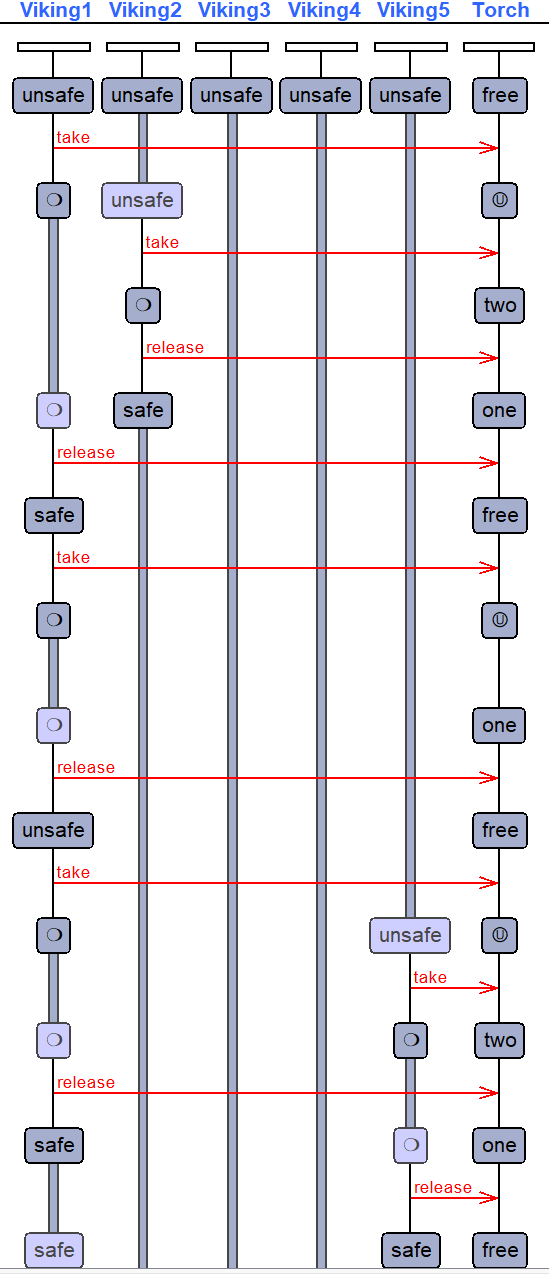
\includegraphics[width=\linewidth,height=0.65\textheight,keepaspectratio]{PartA-2-first.png}
\else
  \fbox{\parbox[c][45mm][c]{\linewidth}{\centering omitted}}
\fi
\caption{First segment.}
\label{fig:parta_a2_first}
\end{subfigure}\hfill
\begin{subfigure}[t]{0.32\textwidth}
\centering
\ifshowimages
  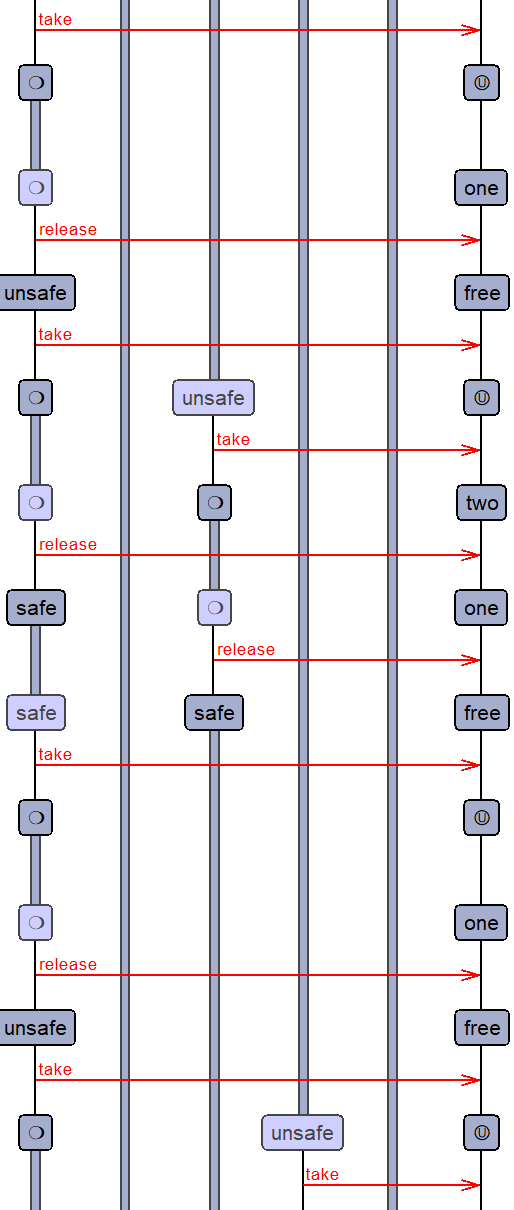
\includegraphics[width=\linewidth,height=0.65\textheight,keepaspectratio]{PartA-2-second.png}
\else
  \fbox{\parbox[c][45mm][c]{\linewidth}{\centering omitted}}
\fi
\caption{Second segment.}
\label{fig:parta_a2_second}
\end{subfigure}\hfill
\begin{subfigure}[t]{0.32\textwidth}
\centering
\ifshowimages
  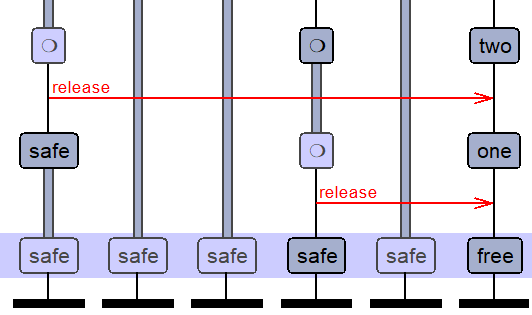
\includegraphics[width=\linewidth,height=0.65\textheight,keepaspectratio]{PartA-2-third.png}
\else
  \fbox{\parbox[c][45mm][c]{\linewidth}{\centering omitted}}
\fi
\caption{Third segment.}
\label{fig:parta_a2_third}
\end{subfigure}
\caption{A.2: UPPAAL simulator trace split across three views.}
\label{fig:parta_a2_strip}
\end{figure}

\subsection*{A.3: Bridge and valley scenario}
\textit{Building on A.2, each Viking may use a longer valley path (no torch; valley delay is $4\times$ each Viking's bridge delay). The bridge still carries two Vikings; the valley has unlimited capacity. What is the shortest time for all five to reach the safe side? Include a schedule with a column indicating bridge vs.\ valley.}
\afterprompt
The soldier template gains a valley location with clock $y$ and invariant $y \le 4\cdot\texttt{delay}$, matching the lab requirement that the valley takes four times as long as the bridge for each Viking. Verification uses bounded reachability, e.g.\
\begin{lstlisting}[style=uppaal]
E<> Vik_1.safe && Vik_2.safe && Vik_3.safe && Vik_4.safe && Vik_5.safe && time <= 40
\end{lstlisting}
The shortest time for all five to reach the safe side in this model is \SI{40}{min}. In the symbolic trace used for the table, $\Vik{3}$ and $\Vik{4}$ cross the bridge together while $\Vik{1}$, $\Vik{2}$, and $\Vik{5}$ (the two \SI{10}{min} Vikings) take the valley concurrently at $t=0$.

\begin{table}[H]
\centering
\begin{tabular}{c >{\raggedright\arraybackslash}p{0.34\textwidth} c c c}
\toprule
\# & Trip (Vikings by index; times in minutes) & Start time (\si{min}) & Trip origin & Bridge or valley \\
\midrule
1 & $\Vik{3}+\Vik{4}$ cross (20+25) & 0 & Unsafe side & bridge \\
2 & $\Vik{1}$ crosses (5) & 0 & Unsafe side & valley \\
3 & $\Vik{2}$ crosses (10) & 0 & Unsafe side & valley \\
4 & $\Vik{5}$ crosses (10) & 0 & Unsafe side & valley \\
\bottomrule
\end{tabular}
\caption{A.3 schedule excerpt (parallel starts at $t=0$ where applicable).}
\label{tab:a3_schedule}
\end{table}

\begin{figure}[H]
\centering
\ifshowimages
  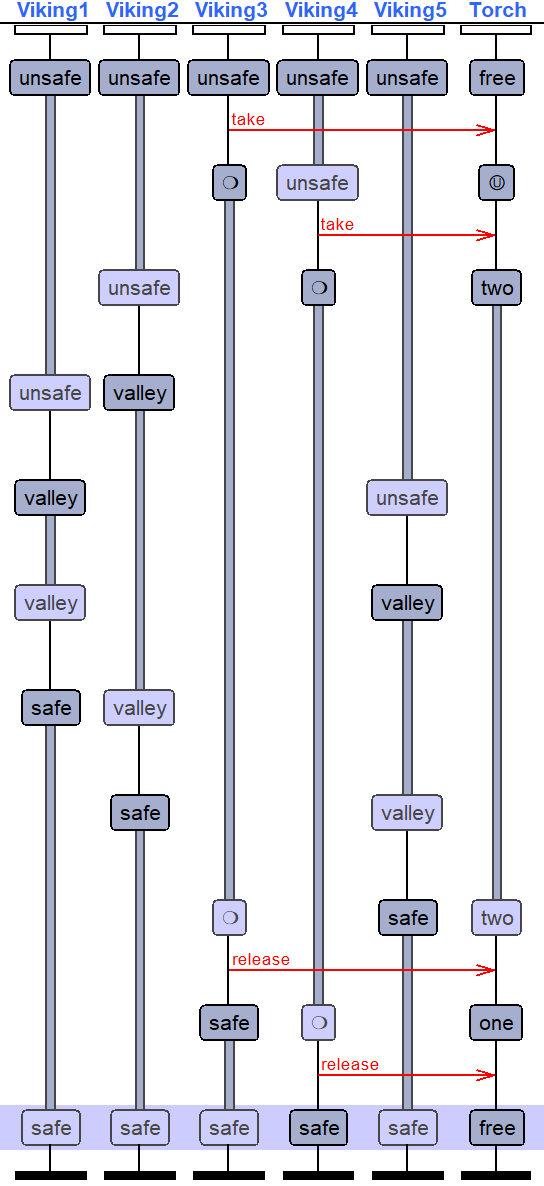
\includegraphics[width=0.88\textwidth,height=0.55\textheight,keepaspectratio]{PartA-3-sim.png}
\else
  \fbox{\parbox[c][42mm][c]{0.88\textwidth}{\centering Image omitted (A.3 sim)}}
\fi
\caption{A.3: UPPAAL simulation/symbolic trace for the bridge--valley model.}
\label{fig:parta_a3_sim}
\end{figure}

\section{Part B: Traffic-Light and Crosswalk Verification}

\subsection*{B.1: Discrete-model reasoning (before timed implementation)}
For each property, a reachability-oriented check was defined conceptually and then evaluated by model intuition over the discrete behavior (no tool reachability on the discrete model in this step).
\medskip

\begin{table}[H]
\centering
\footnotesize
\setlength{\tabcolsep}{2.5pt}
\begin{tabular}{>{\raggedright\arraybackslash}p{0.05\textwidth} >{\raggedright\arraybackslash}p{0.26\textwidth} >{\centering\arraybackslash}p{0.09\textwidth} >{\raggedright\arraybackslash}p{0.54\textwidth}}
\toprule
Prop. & Reachability check idea & Expected truth & Rationale (intuition) \\
\midrule
(a) & It is impossible for the traffic light to be in the pending state \SI{70}{s} after the initial condition. & False & The claim of impossibility is false: pending at \texttt{globalTime==70} can occur if a pedestrian presses the button shortly before the end of a green phase, leaving the controller in pending around that horizon. \\
(b) & It is possible for the traffic and crosswalk lights to be green at the same time. & False & Simultaneous green on both is not expected in normal signaling; the discrete interaction does not support both-green overlap. \\
(c) & The traffic light will never stay in the green (non-pending) location longer than \SI{120}{s}. & True & Timing guards/invariants cap the green phase at \SI{120}{s} or below. \\
(d) & The traffic light will never stay in the pending location for \SI{45}{s} or longer. & False & Pending can persist for up to about \SI{60}{s} in plausible behaviors, so occupying pending for at least \SI{45}{s} is reachable. \\
(e) & The traffic light will never stay in the pending location for \SI{65}{s} or longer. & True & The structure of pending timing prevents occupancy at or above \SI{65}{s}. \\
(f) & It is possible that the crosswalk is red while the traffic light is green. & True & This phase is part of normal operation (e.g., before pedestrian service). \\
(g) & Whenever the crosswalk is red, the traffic light must be green. & False & The model does not enforce this implication; all-red/yellow transitional states break it. \\
(h) & The 3rd occurrence of \texttt{sigG} must not happen within the first \SI{300}{s} after the initial condition. & False (violated) & A third \texttt{sigG} can occur before \SI{300}{s} under fast cycling. \\
(i) & The 3rd occurrence of \texttt{sigG} must not happen within the first \SI{400}{s} after the initial condition. & False (violated) & A third \texttt{sigG} can still occur within \SI{400}{s}; the property is violated similarly to~(h). \\
\bottomrule
\end{tabular}
\caption{B.1 qualitative checks and expected outcomes (intuition only).}
\label{tab:b1_discrete}
\end{table}

\subsection*{B.2: Timed automata model construction}
The timed UPPAAL model includes:
\begin{itemize}
\item Traffic-light and crosswalk-light automata connected by broadcast/synchronization channels (e.g., \texttt{sigR}, \texttt{sigG}, \texttt{sigY}, \texttt{pedG}, \texttt{pedR}).
\item Non-deterministic pedestrian input trigger (\texttt{pedinput}): implemented as a self-looping transmitter so that the pedestrian button channel can fire concurrently with other synchronizations. The self-loop does not encode meaningful defaulting behavior; it exists so that UPPAAL's channel semantics allow the input to be offered in the same step as other transitions when needed.
\item Receiver/sink automata for outputs that would otherwise lack a listener: unused outputs are connected to simple self-looping receivers that absorb signals, which keeps broadcast sends from blocking the rest of the model.
\item Urgent intermediate locations where needed to split transitions that conceptually combine input and output events.
\end{itemize}

The model was exercised with concrete simulation and simple reachability checks before formal verification in B.3.

\labfigure[0.88]{PartB-b2-trafficsys.png}{Timed automata for the traffic-light system (B.2).}{fig:b2_traffic}
\labfigure[0.88]{PartB-b2-pedsys.png}{Crosswalk / pedestrian-side signal system (B.2).}{fig:b2_crosswalk}
\labfigure[0.36]{PartB-b2-pedinput.png}{Non-deterministic \texttt{pedinput} trigger (self-loop for channel firing). Image width is half of the first two B.2 figures.}{fig:b2_pedinput}
\labfigure[0.36]{PartB-b2-receivers.png}{Receiver/sink automata for unused outputs. Image width is half of the first two B.2 figures.}{fig:b2_receivers}
\labfigure[0.75]{PartB-b2-checking_deadlock.png}{Reachability / sanity checks used while testing the B.2 model.}{fig:b2_deadlock}

\subsection*{B.3: Query mapping and verification outcomes}
Each B.1 English statement was translated into a UPPAAL query over the B.2 timed model. The verifier panel confirms results for all checks in one model snapshot.

\begin{table}[H]
\centering
\footnotesize
\begin{tabular}{>{\raggedright\arraybackslash}p{0.06\textwidth} >{\raggedright\arraybackslash}p{0.48\textwidth} >{\centering\arraybackslash}p{0.14\textwidth} >{\centering\arraybackslash}p{0.12\textwidth}}
\toprule
Prop. & Representative UPPAAL query form & UPPAAL outcome & Satisfied (true/false) \\
\midrule
(a) & \texttt{E<> (globalTime==70 \&\& traffic.pending)} & Reachable & true \\
(b) & \texttt{E<> (traffic.green \&\& crosswalk.green)} & Reachable & true \\
(c) & \texttt{A[] (traffic.green imply tGreen<=120)} & Satisfied & true \\
(d) & \texttt{A[] not (traffic.pending \&\& tPend>=45)} & Violated & false \\
(e) & \texttt{A[] not (traffic.pending \&\& tPend>=65)} & Satisfied & true \\
(f) & \texttt{E<> (traffic.green \&\& crosswalk.red)} & Reachable & true \\
(g) & \texttt{A[] (crosswalk.red imply traffic.green)} & Violated & false \\
(h) & \texttt{A[] (sigGCount<3 or globalTime>300)} & Violated & false \\
(i) & \texttt{A[] (sigGCount<3 or globalTime>400)} & Violated & false \\
\bottomrule
\end{tabular}
\caption{B.3 query mapping, UPPAAL outcome, and Boolean satisfaction of the checked formula (true if the query is satisfied in UPPAAL).}
\label{tab:b3_queries}
\end{table}

\noindent\textit{Note.} Property~(b) is marked reachable here; if the discrete intuition in Table~\ref{tab:b1_discrete} suggested otherwise, the timed B.2 model should be treated as authoritative for B.3.

\labfigure[0.92]{PartB-b3-queries.png}{Verifier window: B.3 queries with pass/fail indicators.}{fig:b3_verifier}

\subsection*{B.4: Pedestrian component and unsafe crossing-time range}
The previous button-generator and \texttt{pedG} receiver were replaced with an explicit pedestrian automaton having three locations: \textit{Idle}, \textit{Waiting}, and \textit{Crossing}. Parameter \texttt{pedCrossTime} controls required crossing time.

Bad condition: the system is unsafe when traffic becomes green while the pedestrian remains in the crossing location.

Observed threshold: reachability checks show the bad condition is unreachable at \texttt{pedCrossTime=59} but reachable at \texttt{pedCrossTime=60}. The smallest unsafe value is therefore 60, and values $\geq 60$ are unsafe for this model.

\labfigure[0.82]{PartB-b4-pedsys.png}{Pedestrian template with \texttt{pedCrossTime} and crossing-state timing (B.4).}{fig:b4_ped_model}

\begin{figure}[H]
\centering
\ifshowimages
  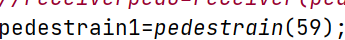
\includegraphics[width=0.48\textwidth]{PartB-b4-at59_clause.png}\\[0.6em]
  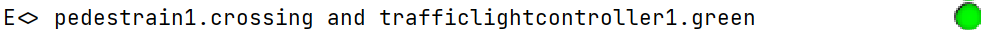
\includegraphics[width=0.48\textwidth]{PartB-b4-at59.png}
\else
  \fbox{\parbox[c][28mm][c]{0.48\textwidth}{\centering omitted}}\par\vspace{0.6em}
  \fbox{\parbox[c][28mm][c]{0.48\textwidth}{\centering omitted}}
\fi
\caption{B.4 safe case at \texttt{pedCrossTime=59}: query/clause (top) and trace (bottom).}
\label{fig:b4_safe59_pair}
\end{figure}

\begin{figure}[H]
\centering
\ifshowimages
  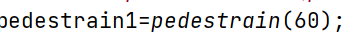
\includegraphics[width=0.48\textwidth]{PartB-b4-at60_clause.png}\\[0.6em]
  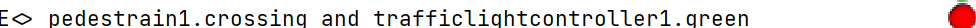
\includegraphics[width=0.48\textwidth]{PartB-b4-at60.png}
\else
  \fbox{\parbox[c][28mm][c]{0.48\textwidth}{\centering omitted}}\par\vspace{0.6em}
  \fbox{\parbox[c][28mm][c]{0.48\textwidth}{\centering omitted}}
\fi
\caption{B.4 unsafe case at \texttt{pedCrossTime=60}: query/clause (top) and trace (bottom).}
\label{fig:b4_unsafe60_pair}
\end{figure}

\subsection*{B.5 (ECE 622): Robustness change for arbitrary crossing time}
\textit{Lab~2 asks for a more robust model such that safety holds regardless of how long the pedestrian takes to cross; explain the change; repeat the B.4 safety query at a \texttt{pedCrossTime} value that was unsafe before and show it is safe after the change; submit \texttt{\_b5.xml} with the report.}
\afterprompt
To remove dependence on a bounded pedestrian crossing duration, a synchronization signal \texttt{done} was introduced from the pedestrian automaton to the traffic controller. The controller defers returning to green until the pedestrian reports crossing completion.

The previously unsafe test point from B.4 (\texttt{pedCrossTime=60}) becomes safe after adding the \texttt{done} handshake and updating controller guards accordingly.

\labfigure[0.84]{PartB-b5-traffic.png}{Traffic controller with \texttt{done} handshake (B.5).}{fig:b5_traffic}
\labfigure[0.84]{PartB-b5-ped.png}{Pedestrian model cooperating with \texttt{done} (B.5).}{fig:b5_ped}
\labfigure[0.55]{PartB-b5-at60.png}{B.5: safety re-check at \texttt{pedCrossTime=60} (now safe).}{fig:b5_at60}
\labfigure[0.55]{PartB-b5-at60_clause.png}{B.5: corresponding query/clause for the unsafe condition at \texttt{pedCrossTime=60}.}{fig:b5_at60_clause}
\labfigure[0.72]{PartB-b5-crossed_allow_at60.png}{B.5: additional confidence checks (e.g.\ crossing allowed under robust model).}{fig:b5_crossed}

\begin{table}[H]
\centering
\footnotesize
\setlength{\tabcolsep}{3pt}
\begin{tabular}{>{\raggedright\arraybackslash}p{0.04\textwidth} >{\raggedright\arraybackslash}p{0.30\textwidth} >{\raggedright\arraybackslash}p{0.54\textwidth} >{\centering\arraybackslash}p{0.06\textwidth}}
\toprule
\# & Lab~2 B.5 requirement (paraphrase) & What this report demonstrates & OK? \\
\midrule
1 & Robust model: safe regardless of crossing duration. & \texttt{done} handshake; green deferred until crossing completes (Figs.~\ref{fig:b5_traffic}--\ref{fig:b5_ped}). & Y \\
2 & Explain the change in the report. & Text and figures; \texttt{done} removes reliance on a fixed \texttt{pedCrossTime} for safety. & Y \\
3 & Repeat B.4 safety query at a previously unsafe \texttt{pedCrossTime}; show safe after change. & Figs.~\ref{fig:b5_at60}--\ref{fig:b5_at60_clause}: bad condition unreachable at \texttt{pedCrossTime=60}. & Y \\
4 & Simulate / use extra queries for confidence. & Fig.~\ref{fig:b5_crossed} and B.2-style checks. & Y \\
5 & Submit \texttt{\_b5.xml} with the report. & Course-style filename (e.g.\ \texttt{*\_b5.xml}) included with submission materials. & Y \\
\bottomrule
\end{tabular}
\caption{B.5 alignment checklist: lab wording vs.\ evidence in this report (for grading).}
\label{tab:b5_alignment}
\end{table}

\section*{Conclusion}
This lab demonstrates how UPPAAL supports rigorous analysis of both scheduling and reactive control problems. In Part~A, bounded reachability and trace extraction were used to derive crossing schedules under increasingly rich constraints. In Part~B, timed automata and formal queries were used to relate informal predictions to tool results, to expose unsafe regimes, and to validate a robustness refinement that removes dependence on a fixed pedestrian timing assumption.

\end{document}
